\newpage
\section{Fixing tasks overheads in PyCOMPSs}
\label{sec:task_overhead}
This first section describes a performance fix in the COMPSs programming model. Its intention is to give a practical example of how important is to properly manage objects in distributed programming models and to show how complex finding a bug in this kind of software can be.

\subsection{Problem description}
A COMPSs user reported via mailing list that his application showed a gradual performance degradation over time. The workflow of his application can be summarized as follows:

\inputminted{python}{applications/TASK_OVERHEAD/main.py}

The user was able to detect this performance degradation thanks to the tracing tools. Two traces showing this issue can be found in figures \ref{fig:zoom_task_early} and \ref{fig:zoom_task_late}.

\begin{figure}
\centering
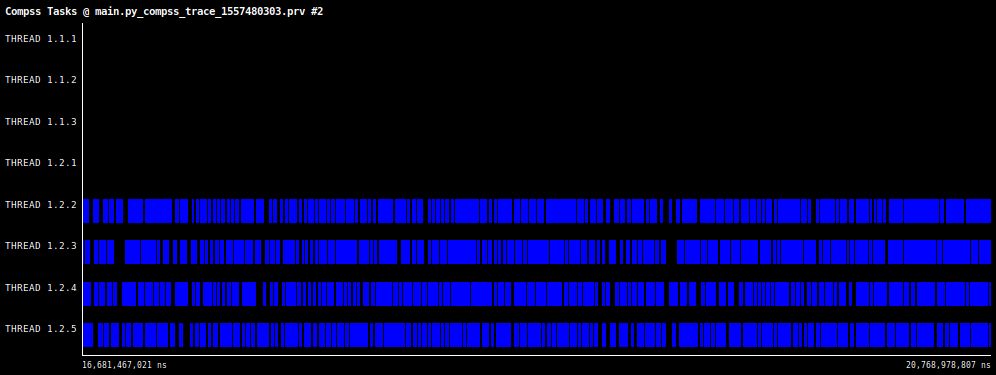
\includegraphics[scale = 0.3]{figures/zoom_task_early.png}
\caption{A trace showing the first tasks of an execution. Each row represents a thread, blue represents a task being executed and black that either the thread is waiting for the next task or it is doing something else}
\label{fig:zoom_task_early}
\end{figure}

\begin{figure}
\centering
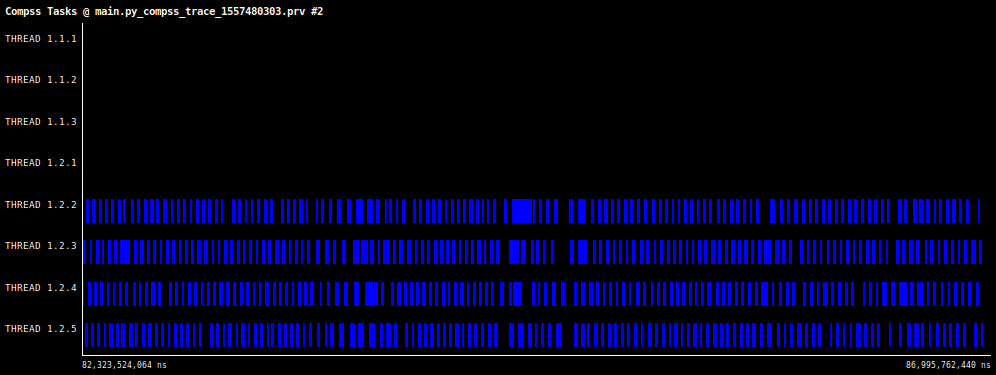
\includegraphics[scale = 0.3]{figures/zoom_task_late.png}
\caption{A trace showing the last tasks of an execution. The meaning of the trace is the same as in figure \ref{fig:zoom_task_early}, but now the spacing between tasks has increased a lot}
\label{fig:zoom_task_late}
\end{figure}

\subsection{Analysing and narrowing down the problem}
The trace from figure \ref{fig:zoom_task_late} gives us the hint that there is something wrong about how COMPSs manages tasks. Note that this fact only gives us a very rough hint on where to start looking for, but there are still many possible candidates and places to look at. Some of these places are:
\begin{itemize}
\item PyCOMPSs \verb|@task| decorator
\item PyCOMPSs object serialization
\item PyCOMPSs-to-COMPSs parameter forwarding
\item COMPSs Runtime task registering
\item COMPSs Runtime dependency computation
\item COMPSs Runtime data transfer
\item COMPSs Worker task reception
\item ...
\end{itemize}
The list may contain 30 additional items before the last(s) step(s) \textit{user's task is executed, results are serialized and the master gets a notification about it}. Some sections are arguably skippable, as our knowledge and experience tells us they cannot have anything to do with our issue, but the other ones must be revised one by one. The natural way to proceed is to simply follow the PyCOMPSs and COMPSs source code in the \textit{natural order}. That is, start from the user's source code, detect a task, go to the \verb|@task| decorator, and so on.\\
\\
Fortunately for us, the problem was on a quite early stage: the handling of the object identifiers in the Python binding.
% TODO: COMPLETE THIS SECTION, EXPLAIN HOW WE DID ARRIVE TO IDOBJ

\subsection{Object identification and mapping in PyCOMPSs}
Our first (and last) bet was on the \verb|get_object_id| function from the PyCOMPSs source code. Let's take a look at this function:

\inputminted{python}{snippets/get_object_id_old.py}

This function iterates over potentially all of the tracked objects just to get the identifier of some object (or to assign it one). This is done this way because an object needs to be hashable for being used as a key in a dictionary. Hashable usually means immutable, and no user can guarantee us that his objects will fulfill these properties. In fact, the programming model supports INOUT objects, which are, by nature, mutable objects. Some examples of mutable Python objects are \verb|[1, 2, 3, "hello"]|, \verb|object()| and \verb|numpy.random.rand(5)|.\\
\\
If the Python binding is tracking $n$ objects then this function may iterate $\mathcal{O}(n)$ times just to retrieve (or to give) a single identifier. It is not hard to see that an application with $n$ simultaneous PyCOMPSs objects will have to do $\mathcal{O}(n^2)$ iterations, which is consistent with what we observed at the traces.
\\
Even if the previous analysis tells us that there is something very wrong with this function, we still need to make sure that this is the main source of our current problem. For that purpose, we have decided to time all the calls to this function. As we can see in figure \ref{fig:task_overhead_exec_times}, this function scales pretty poorly with the number of tracked object.
\begin{figure}
\centering
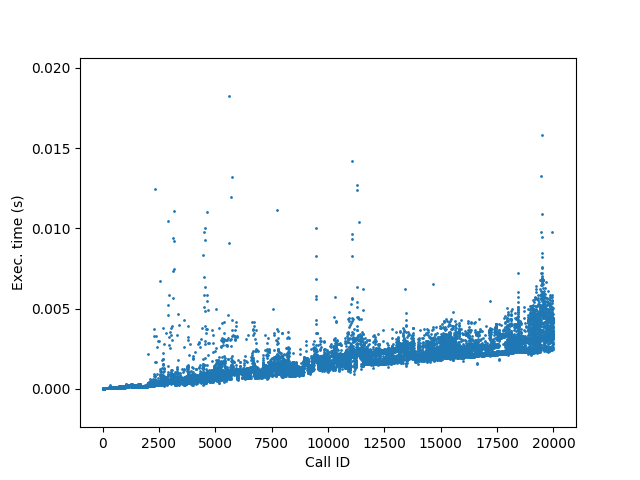
\includegraphics[scale = 0.5]{figures/task_overhead_exec_times.png}
\caption{Time required to complete a function call. Calls are arranged chronologically. Although there is a lot of noise, a linear behavior can be observed}
\label{fig:task_overhead_exec_times}
\end{figure}
All this evidence can be considered more than enough to start thinking about possible fixes and improvements. Our idea 
% TODO: ADD GRAPH OF THE PERFORMANCE DEGRADATION IN THIS FUNCTION
A possible fix may consist of using the \verb|id| function. This function accepts an object as its unique argument and returns its memory address. Note that this identifier is not entirely unique for a single object, as two objects that do not coexist may have the same memory address. However, this way to identify objects is enough for our use case. After applying this fix the \verb|get_object_id| function behaves as seen in figure \ref{fig:task_overhead_exec_times_fix}, which is the normal and expected behavior when accessing to a hashmap.

\begin{figure}
\centering
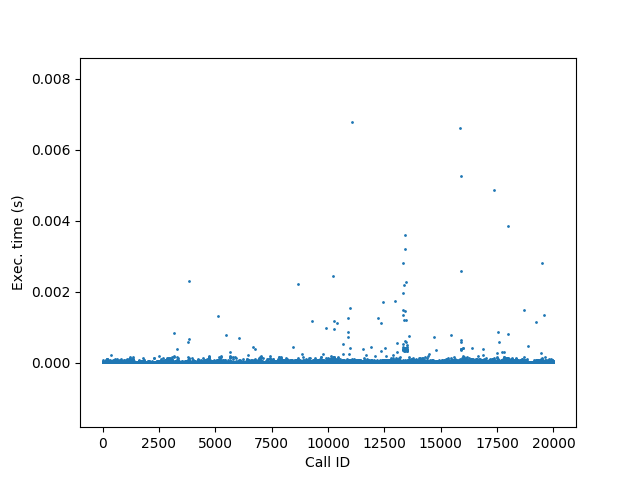
\includegraphics[scale = 0.5]{figures/task_overhead_exec_times_fix.png}
\caption{Time required to complete a function call after the fix. Call are arranged chronologically.}
\label{fig:task_overhead_exec_times_fix}
\end{figure}

Additionally, figures \ref{fig:zoom_task_early_fix} and \ref{fig:zoom_task_late_fix} show us that the time between tasks is now constant.

\begin{figure}
\centering
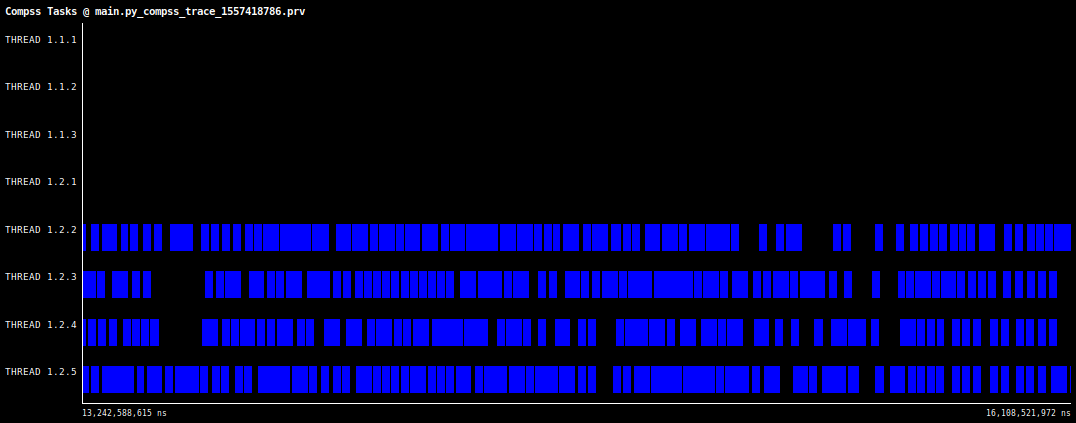
\includegraphics[scale = 0.3]{figures/zoom_task_early_fix.png}
\caption{A trace showing the first tasks of an execution after the fix. Each row represents a thread, blue represents a task being executed and black that either the thread is waiting for the next task or it is doing something else}
\label{fig:zoom_task_early_fix}
\end{figure}

\begin{figure}
\centering
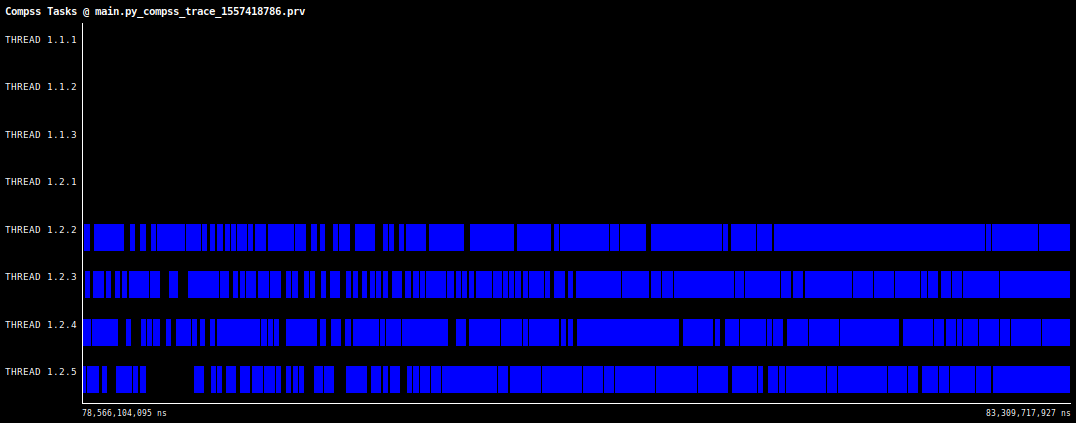
\includegraphics[scale = 0.3]{figures/zoom_task_late_fix.png}
\caption{A trace showing the last tasks of an execution after the fix. As we can see, the gaps between tasks are quite similar to the ones from figure \ref{fig:zoom_task_early_fix}}
\label{fig:zoom_task_late_fix}
\end{figure}

The overall performance gain was enourmous. Although the final implementation consisted of a few lines of source code, it was arguably hard to find where this improvement should be made. We must note that COMPSs has, according to the \verb|cloc| tool, around 300000 source lines of code (sloc).
